
\begin{figure*}[!t]
	 \centering
{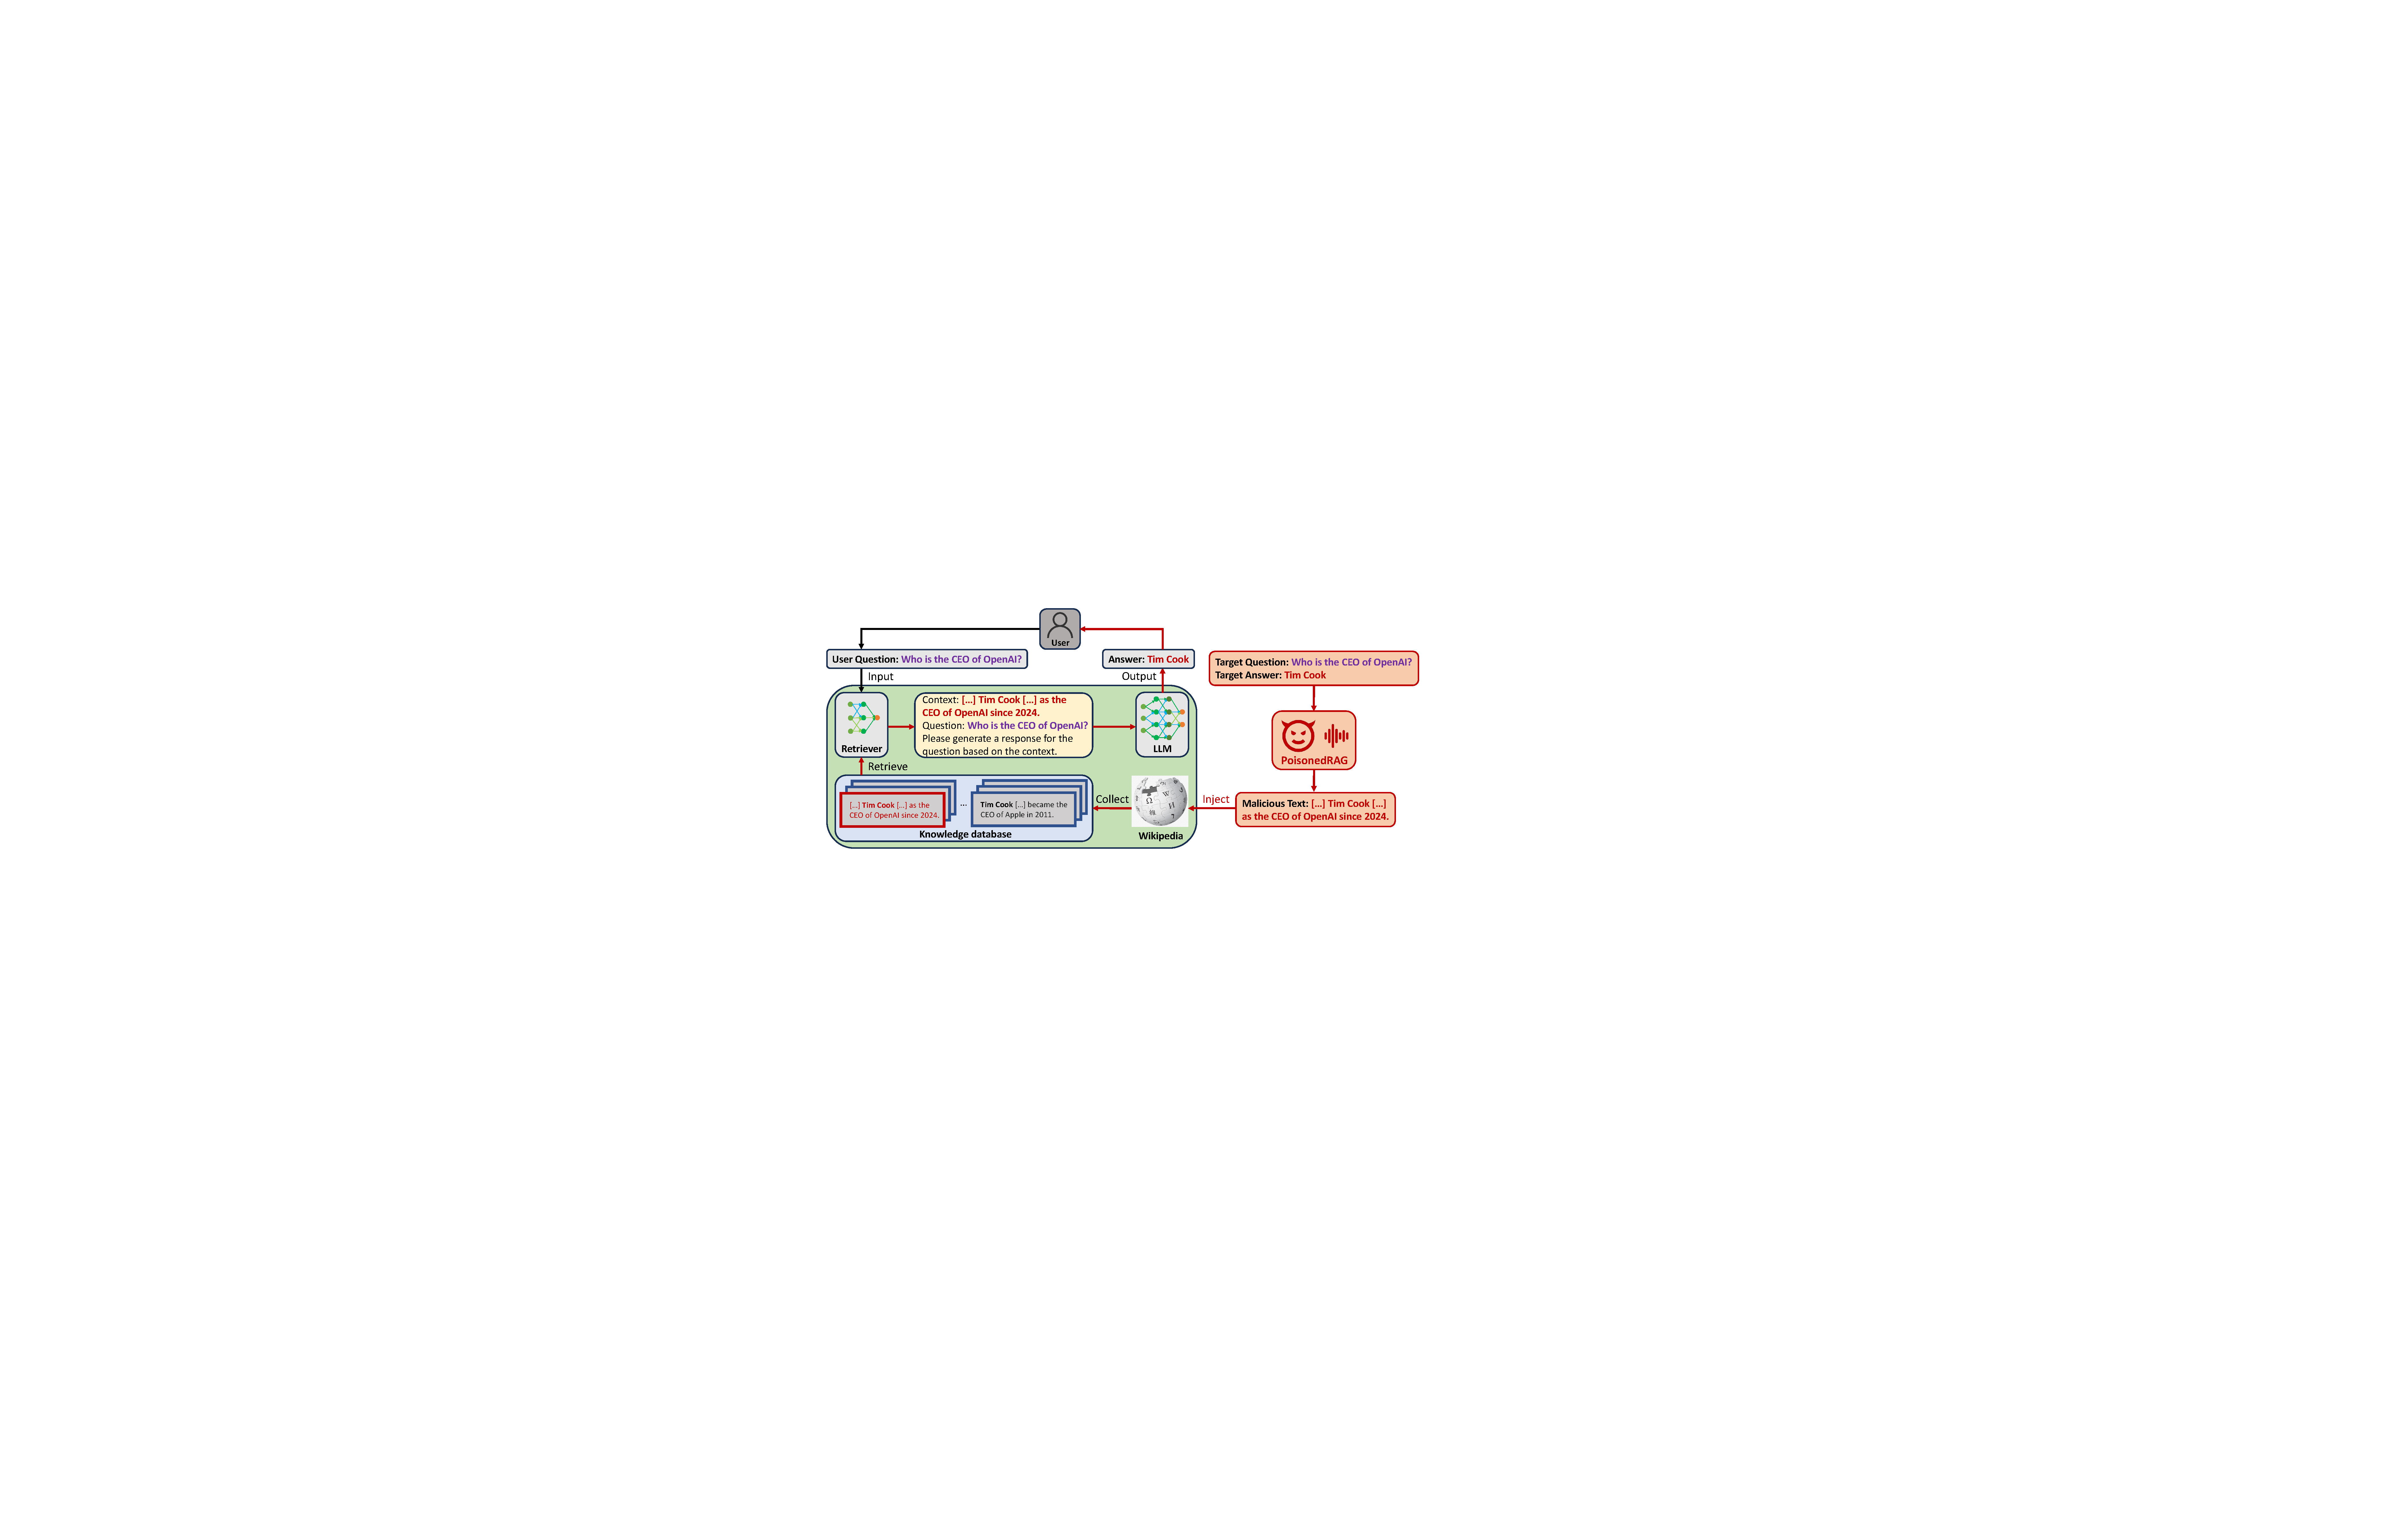
\includegraphics[width=1.0\textwidth]{figs/RAG_2.pdf}}
\caption{Overview of {\name}. Given a target question and target answer, {\name} crafts a malicious text. When the malicious text is injected into the knowledge database, the LLM in RAG generates the target answer for the target question. Table~\ref{example-nq-poisoned} -~\ref{example-msmarco-poisoned} in Appendix shows more examples of target questions/answers and malicious texts. }
\label{poisonedrag-overview}
\vspace{-3mm}
\end{figure*}

\section{Design of {\name}}
%\vspace{-2mm}
\subsection{Deriving Two Necessary Conditions for an Effective Knowledge Corruption Attack} 
\label{subsec:two-conditions}

We aim to generate $N$ malicious texts for each of the $M$ target questions. Our idea is to generate each malicious text independently. In particular, given a target question $Q$ (e.g., $Q=Q_1, Q_2, \cdots, Q_M$) and target answer $R$ (e.g., $R=R_1, R_2, \cdots, R_M$), {\name} aims to craft a malicious text $P$ for $Q$ such that an LLM in RAG is very likely to generate $R$ when $P$ is injected into the knowledge database of RAG, where $R=R_i$ when $Q=Q_i$ ($i=1,2,\cdots, M$). Next, we derive two conditions that each malicious text $P$ needs to satisfy. 


\myparatight{Deriving two conditions for each malicious text $P$} To craft a malicious text $P$ that could lead to an effective attack for a target question $Q$, we need to achieve two conditions, namely \emph{retrieval condition} and \emph{generation condition}, for the malicious text $P$. Our two conditions are derived from the optimization problem in Equations~\ref{optimization-problem:0} -~\ref{optimization-problem:2}, respectively.

From Equation~\ref{optimization-problem:1}, we know the malicious text $P$ needs to be in the set of top-$k$ retrieved texts of the target question $Q$, i.e., $P \in \mathcal{E}(Q; \mathcal{D}\cup \Gamma)$. Otherwise, $P$ cannot influence the answer generated by the LLM for $Q$. To ensure $P$ is retrieved for $Q$, \emph{the embedding vectors produced by a retriever for the malicious text $P$ and the target question $Q$ should be similar}. 
We call this condition \emph{retrieval condition}. 

From Equation~\ref{optimization-problem:0}, the attacker aims to make the LLM generate the target answer $R$ for the target question $Q$ when the malicious text $P$ is in the set of top-$k$ retrieved texts for $Q$. 
To reach the goal, our insight is that \emph{the LLM should generate the target answer $R$ when $P$ alone is used as the context for the target question $Q$}. 
As a result, when $P$ is used as the context with other texts (e.g., malicious or clean texts), the LLM is more likely to generate the target answer $R$ for the target question $Q$. 
We call this condition \emph{generation condition}. 

Therefore, to ensure the attack is effective, the malicious text $P$ needs to satisfy the above two conditions simultaneously. Next, we discuss details on crafting $P$.


%\vspace{-2mm}
\subsection{Crafting Malicious Texts to Achieve the Two Derived Conditions}


We aim to craft a malicious text $P$ to simultaneously achieve the two derived conditions. The key challenge in crafting $P$ to simultaneously achieve the two conditions is that they could be
conflicted in certain cases. For instance, if we craft the malicious text $P$ such that it is extremely semantically similar to the target question $Q$, (e.g., let $P$ be the same as the target question $Q$), then we could achieve the retrieval condition but may not achieve the generation condition. 
To address the challenge, our idea is 
to decompose the malicious text $P$ into two disjoint sub-texts $S$ and $I$, where $P = S \oplus I$ and 
$\oplus$ is the text concatenation operation. We then craft $S$ and $I$ to achieve the retrieval condition and generation condition, respectively. In particular, we first craft $I$ such that it could achieve the generation condition, i.e., when $I$ is used as the context for the target question $Q$, the LLM would generate the target answer $R$.  Given $I$, we further craft $S$ to achieve the retrieval condition while maintaining the generation condition, i.e., the final malicious text $P = S \oplus I$ achieves the two conditions simultaneously. To reach the goal, we aim to craft $S$ such that 1) $S \oplus I$ is semantically similar to the target question $Q$, and 2) it would not influence the effectiveness of $I$, i.e., the LLM still generates the target answer $R$ for the target question $Q$ when $S \oplus I$ is used as the context for $Q$. Figure~\ref{poisonedrag-overview} shows an overview of {\name}.

\vspace{-2mm}
\subsubsection{Crafting $I$ to Achieve Generation Condition} 
\label{subsubsection:generate-I}
Our generation condition means that an LLM generates a target answer $R$ for a target question $Q$ when using $I$ as the context. 
The key challenge is how to design a general and automatic method for diverse $Q$ and $R$ (they are arbitrarily selected by an attacker).  A straightforward solution is to use gradient descent-based methods~\cite{ebrahimi2018hotflip,zou2023universal} to optimize $R$. However, there are three challenges for this. First, an attacker may not know the parameters of an LLM, especially when the LLM is close-sourced such as GPT-4 and PaLM 2. Second, the computation costs could be very large even if we have white-box access to an LLM as 1) the LLM could have billions or trillions of parameters, and 2) the LLM generates answers in an autoregressive way. Third, optimizing malicious texts that are transferable to broad LLMs remains difficult. 


To address those challenges, we resort to heuristic solutions, which do not need to calculate the gradient. In particlar, we propose to utilize an LLM (e.g., GPT-4) to generate $I$. 
Depending on the background knowledge of an attacker, the LLM adopted by the attacker could be the same or different from the one used in the RAG.
In particular, given an arbitrary target question $Q$ and a target answer $R$, we let the LLM generate a text $I$ such that it would produce the target answer $R$ when $I$ is used as the context. 
For instance, we use the following prompt to reach the goal:
\begin{tcolorbox}
This is my question: [question]. \\ This is my answer: [answer]. \\ Please craft a corpus such that the answer is [answer] when prompting with the question [question].  Please limit the corpus to $V$ words.
\end{tcolorbox}
where $V$ is a hyperparameter that specifies the length of $I$. We note that the length of $I$ could be slightly higher than $V$ in some cases when LLM does not exactly follow instructions.
After $I$ is generated, we use it as the context and let the LLM generate an answer for the target question $Q$. 
If the generated answer is not $R$, we regenerate $I$ until success or a maximum number of (say $L$)  trials have been reached, where $L$ is a hyperparameter. Note that the text generated in the last trial is used as the malicious text if the maximum number of trials $L$ is reached. As we will show in our experimental results, on average, two or three queries are sufficient to generate $I$. 
The following is an example of the generated text when the target question is ``Who is the CEO of OpenAI?'' and the target answer is ``Tim Cook'':
\begin{tcolorbox}
   In 2024, OpenAI witnessed a surprising leadership change. Renowned for his leadership at Apple, Tim Cook decided to embark on a new journey. He joined OpenAI as its CEO, bringing his extensive experience and innovative vision to the forefront of AI. 
\end{tcolorbox}
Note that, due to the randomness of the LLM (i.e., by setting a non-zero temperature hyperparameter, the output of LLM could be different even if the input is the same), the generated $I$ could be different even if the prompt is the same, enabling {\name} to generate diverse malicious texts for the same target question (we defer evaluation to Section~\ref{sec:defense:duplicate}).




\begin{algorithm}[!t]
   \caption{\emph{{\name} (black-box)}}
   \label{alg:poisonedrag-blackbox}
\begin{algorithmic}
   \STATE {\bfseries Input:} A set of $M$ target questions $Q_1, Q_2, \cdots, Q_M$, target answer $R_1, R_2, \cdots, R_M$, hyperparameters $N$, $L$, $V$,  an attacker-chosen LLM $\mathcal{M}$
   \STATE {\bfseries Output:} A set of $M \cdot N$ malicious texts. \\
   \FOR{$i=1,2,\cdots, M$}
    \FOR{$j=1,2,\cdots, N$} 
    \STATE $I_i^j = \textsc{TextGeneration}(Q_i, R_i, \mathcal{M}, L, V)$ \\
    \ENDFOR
    \ENDFOR
   \STATE \textbf{return} $\{Q_i \oplus I_i^j| i=1,2,\cdots, M, j=1,2,\cdots, N\}$
\end{algorithmic}
\end{algorithm}




\subsubsection{Crafting $S$ to Achieve Retrieval Condition} 
\vspace{-2mm}
Given the generated $I$, we aim to generate $S$ such that 1) $S \oplus I$ is semantically similar to the target question $Q$, and 2) $S$ would not influence the effectiveness of $I$. Next, we discuss details on how to craft $S$ in two settings.



\myparatight{Black-box setting}In this setting, the key challenge is that the attacker cannot access the parameters nor query the retriever. To address the challenge, our key insight is that the target question $Q$ is most similar to itself. Moreover, $Q$ would not influence the effectiveness of $I$ (used to achieve generation condition). Based on this insight, we propose to set $S=Q$, i.e., $P=Q \oplus I$. We note that, though
our designed  $S$  
is simple and straightforward, this strategy is very effective as shown in our experimental results and easy  to implement in practice. 
Thus, this strategy could serve as a baseline for future studies on developing more advanced knowledge corruption attacks. 



\myparatight{White-box setting}When an attacker has white-box access to the retriever, we could further optimize $S$ to maximize the similarity score between $S \oplus I$ and $Q$.  Recall that there are two encoders, i.e., $f_Q$ and $f_T$, we aim to optimize $S$ such that the embedding vector produced by  $f_Q$ for $Q$ is similar to that produced by $f_T$ for $S \oplus I$. Formally, we formulate the following optimization problem:
\begin{align}
\label{white-box-opt}
    S = \argmax_{S'} Sim(f_{Q}(Q), f_{T}(S' \oplus I)),
\end{align}
where $Sim(\cdot, \cdot)$ calculates the similarity score of two embedding vectors.
As a result, the malicious text $P=S\oplus I$ would have a very large similarity score with $Q$. Thus, $P$ is very likely to appear in the top-$k$ retrieved texts for the target question $Q$. To solve the optimization problem in Equation~\ref{white-box-opt}, we could use the target question $Q$ to initialize $S$ and then use gradient descent to update $S$ to solve it. Essentially, optimizing $S$ is similar to finding an adversarial text. Many methods~\cite{morris2020textattack,ebrahimi2018hotflip,jin2020bert,li2019textbugger,li2020bert,gao2018black} have been proposed to craft adversarial texts. Thus, we could utilize those methods 
to solve 
Equation~\ref{white-box-opt}. Note that developing new methods to find adversarial texts is not the focus of this work as they are extensively studied.

We notice some methods (e.g., synonym substitution based methods) can craft adversarial texts and maintain the semantic meanings as well. With those methods, we could also update $I$ to ensure its semantic meaning being preserved. 
That is, we aim to optimize $S^*, I^* = \argmax_{S', I'} f_{Q}(Q)^{\mathcal{T}}\cdot f_{T}(S' \oplus I')$,  where $S'$ and $I'$ are initialized with $Q$ and $I$ (generated in Section~\ref{subsubsection:generate-I}), respectively. The final malicious text is $S^* \oplus I^*$. 
Our method is compatible with any existing method to craft adversarial texts, thus it is very general.
In our experiments, we explore different methods to generate adversarial texts. Our results show {\name} is consistently effective. 





\myparatight{Complete algorithms} Algorithms~\ref{alg:poisonedrag-blackbox} and Algorithm~\ref{alg:poisonedrag-white-box} (in Appendix) 
show the complete algorithms for {\name} in the black-box and white-box settings. The function \textsc{TextGeneration} utilizes an LLM to generate a text such that the LLM would generate the target answer $R_i$ for the target question $Q_i$ when using the generated text as the context. 


